
\section{Results}
\label{sec:results}

The main metric used to measure the effectiveness of the ant-based algorithm was the number of calls dropped over the 15,000 time step simulation. We compared our algorithm to breadth-first search as a naiive shortest-path, non-adaptive algorithm, as well as Dijkstra's Algorithm, a least-weight algorithm which we modified to use node weights instead of edge weights.\\

\begin{figure}[htb]
  \centering
  \begin{tabular}{|c|c|c|} 
     \hline % draws two horizontal lines at the top of the table
     & Mean & SD \\ 
    \hline % line after the column headers
    Breadth-First Search & $11.99\%$ & $0.33\%$ \\
    Ant-Based ($0\%$ Noise) & $4.87\%$ & $0.35\%$\\
    Ant-Based ($5\%$ Noise) & $5.24\%$ & $0.40\%$\\
    Dijkstra's Algorithm & $0.11\%$ & $0.04\%$\\
    \hline
  \end{tabular}
  \caption{Percentages of dropped calls over 10 runs of 15,000 time steps.}
  \label{tab:results}

\end{figure}

The call dropping seemed to cycle slightly, as the network became more and less congested. Additionally, with the ant-based algorithm, results seemed to get slightly worse over time, though not severely. 

\begin{figure}[htb]

  \centering
  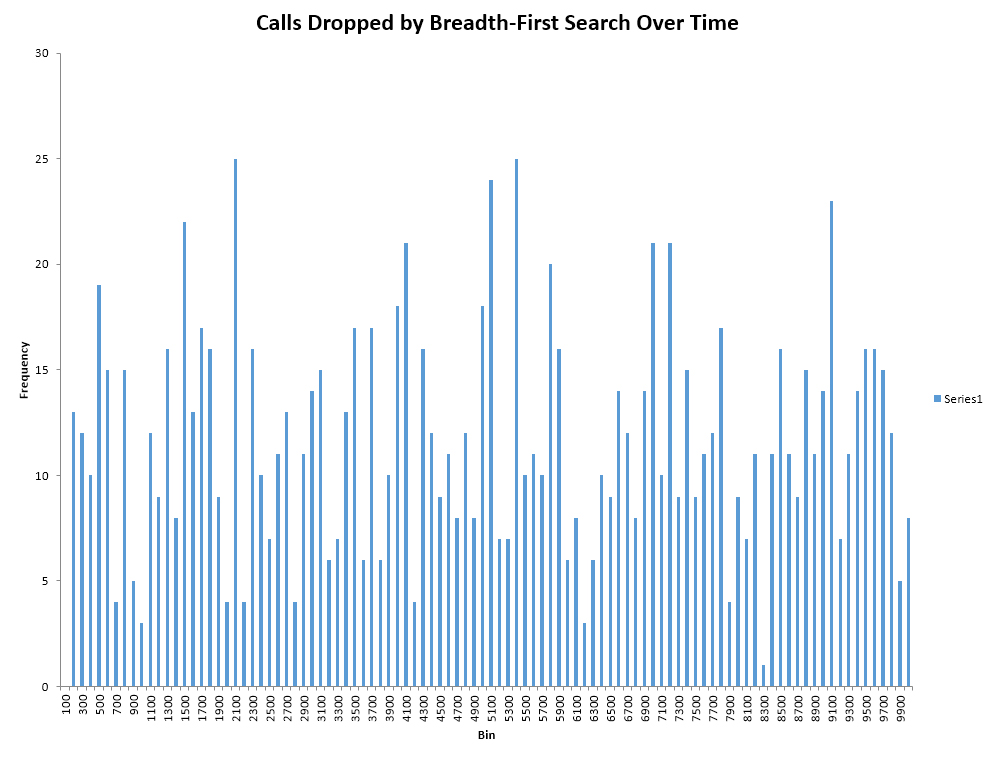
\includegraphics[width=0.47\textwidth]{figs/bfs_hist.jpg}
  \caption{Calls dropped by breadth-first search.}
  \label{fig:bfs_hist}

\end{figure}

\begin{figure}[!h]

  \centering
  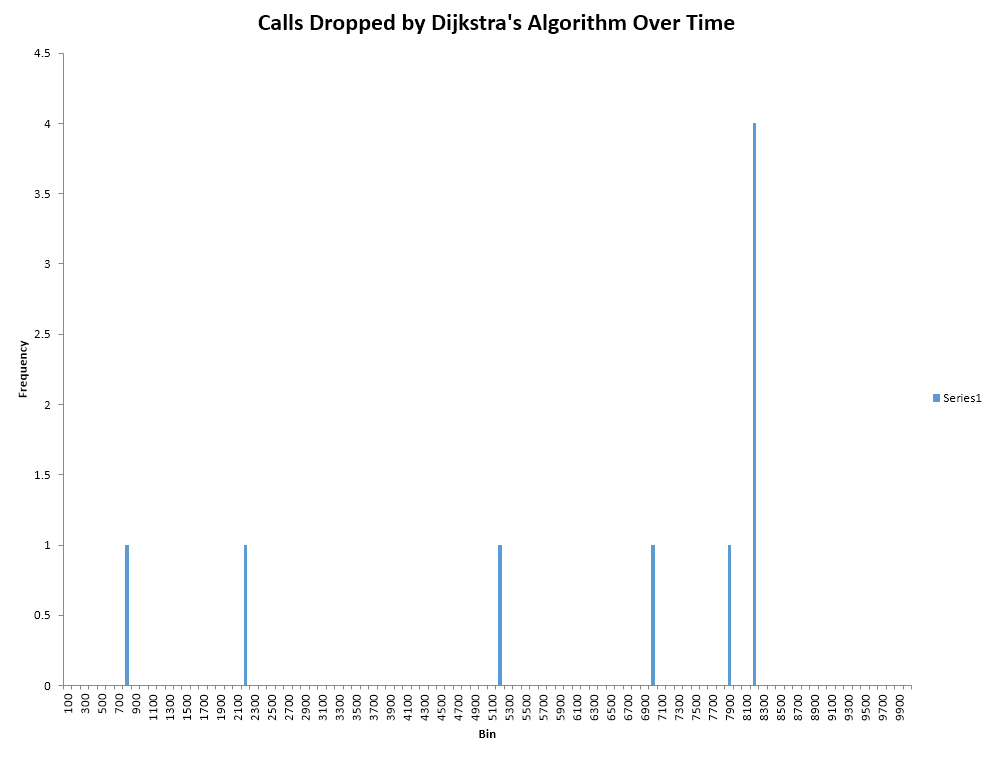
\includegraphics[width=0.47\textwidth]{figs/dijk_hist.jpg}
  \caption{Calls dropped by Dijkstra's algorithm.}
  \label{fig:dijk_hist}

\end{figure}

\begin{figure}[htb]

  \centering
  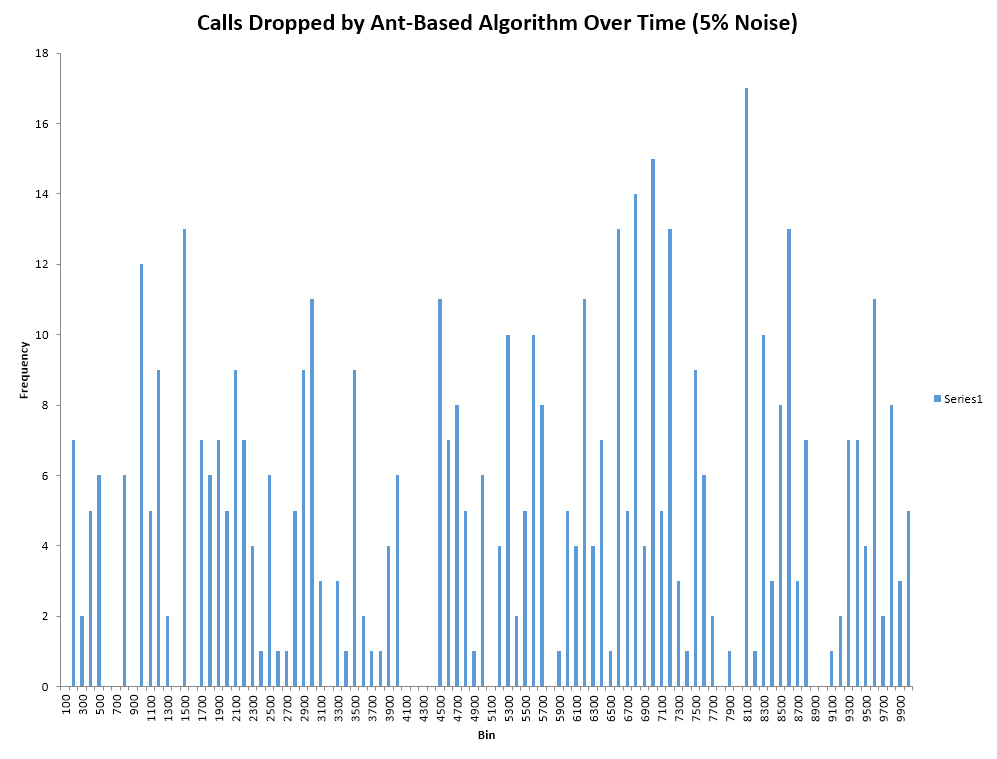
\includegraphics[width=0.47\textwidth]{figs/ant_hist.jpg}
  \caption{Calls dropped by the ant-based algorithm.}
  \label{fig:ant_hist}

\end{figure}

The ant population in this model rose quickly but ended up converging to around 3500 ants. When tested with 100\% noise, the ant population continuously kept climbing, creating an unnecessary processing strain. This is the primary advantage of having ants follow the pheromone trails, it seems; it keeps the ant population at a managable size.

\begin{figure}[htb]

  \centering
  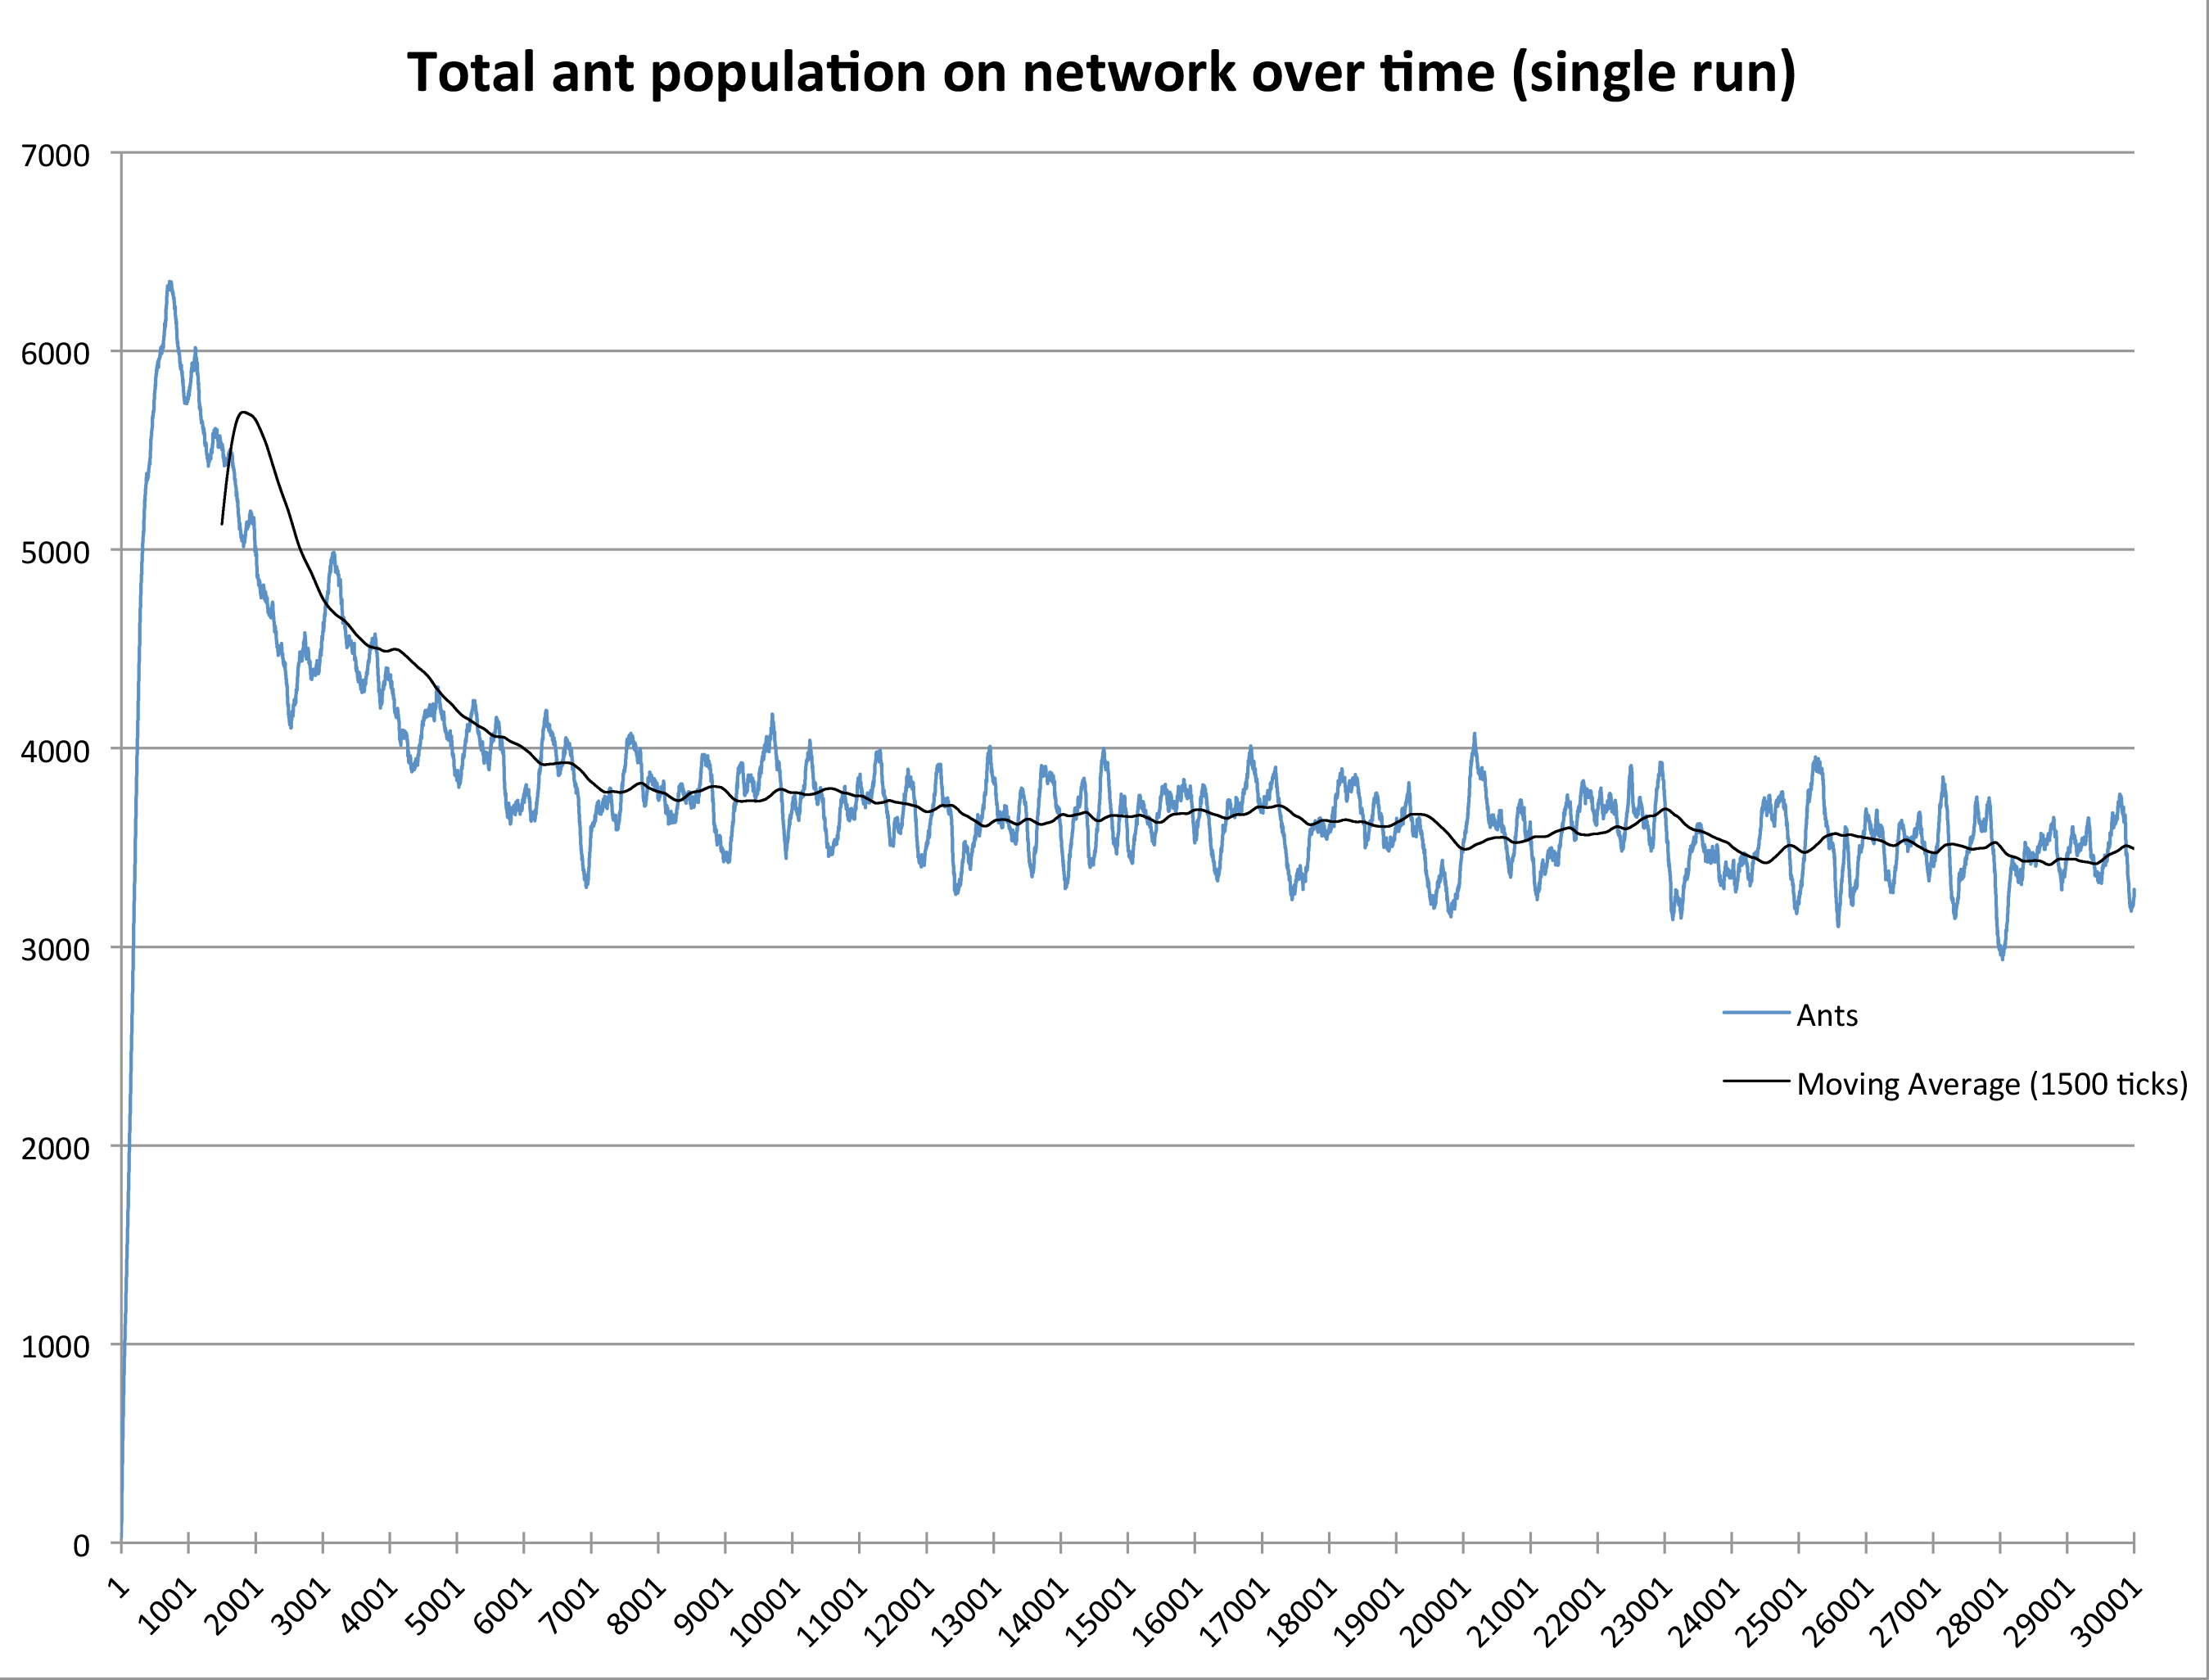
\includegraphics[width=0.47\textwidth]{figs/ant_pop.jpg}
  \caption{Ant population over time.}
  \label{fig:btc}

\end{figure}